\section*{Problema P9.37}

\renewcommand*\thesection{9.37}
\numberwithin{equation}{section}

\begin{center}
    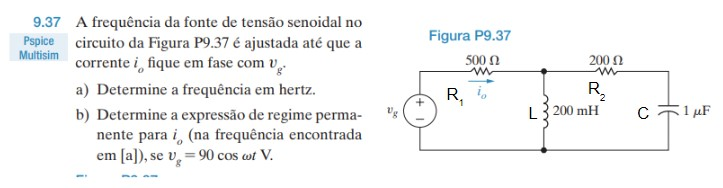
\includegraphics[scale=1.0]{P9.37.jpg}
\end{center}

\subsection*{(a)}

Vamos começar identificando a impedância equivalente \( Z_{in} \) vista pela fonte \( v_g \).

\[ Z_{in} = \left(\left(\frac{1}{j\omega C} + R_2\right) \; // \; j\omega L\right) +  R_1 \]

\[ Z_{in} = R_1 + \frac{1}{\frac{1}{j\omega L} + \frac{1}{\frac{1}{j\omega C} + R_2}}  \]

Agora vamos isolar a parte real da parte complexa.

\[ Z_{in} = R_1 + \frac{1}{-\frac{j}{\omega L} + \frac{1}{-\frac{j}{\omega C} + R_2}}  \]

\[ Z_{in} = R_1 + \frac{1}{-\frac{j}{\omega L} + \frac{\omega C}{-j + R_2\omega C}}  \]

\[ Z_{in} = R_1 + \frac{1}{-\frac{j}{\omega L} + \frac{(\omega C)(+j + R_2\omega C)}{1^2 + (R_2\omega C)^2}}  \]

\[ Z_{in} = R_1 + \frac{1}{-\frac{j}{\omega L} + \frac{j\omega C}{1 + (R_2\omega C)^2} + \frac{R_2\omega^2C^2}{1 + (R_2\omega C)^2} }  \]

\[ Z_{in} = R_1 + \frac{1}{- \frac{R_2\omega^2C^2}{1 + (R_2\omega C)^2} + j\left(-\frac{1}{\omega L} + \frac{\omega C}{1 + (R_2\omega C)^2} \right) }  \]


Vamos adotar uma notação para simplificar a expressão. Sejam

\[ 
    A = \frac{R_2\omega^2C^2}{1 + (R_2\omega C)^2}
    \quad , \quad
    B = - \frac{1}{\omega L} + \frac{\omega C}{1 + (R_2\omega C)^2}
\]

Com isso, podemos reescrever a expressão de \( Z_{in} \) como

\[ Z_{in} = R_1 + \frac{1}{A + jB}  \]

Continuamos o processo de isolar a parte real da parte complexa.

\[ Z_{in} = R_1 + \frac{1}{A + jB}  \]

\[ Z_{in} = R_1 + \frac{A - jB}{A^2 + B^2}  \]

\[ Z_{in} = \left(R_1 + \frac{A}{A^2 + B^2}\right) - j\frac{B}{A^2 + B^2}  \]

Agora é possível expressar uma função para o ângulo de fase \( \phi \) de \( Z_{in} \), dada por

\[ \phi = \tan^{-1}\left(\frac{-\frac{B}{A^2 + B^2}}{R_1 + \frac{A}{A^2 + B^2}}\right) \]

\[ \phi = \tan^{-1}\left(\frac{-\frac{B}{A^2 + B^2}}{\frac{R_1(A^2 + B^2) + A}{A^2 + B^2}}\right) \]

\begin{equation}\label{eq:9.37.1}
    \phi = \tan^{-1}\left(-\frac{B}{R_1(A^2 + B^2) + A}\right)
\end{equation}

Uma vez calculado $Z_{in}$, podemos expressar a relação entre $V_g$ e $I_o$ através de

\begin{equation}\label{eq:9.37.2}
    V_g = Z_{in} \cdot I_g
\end{equation}

Para que (\ref{eq:9.37.2}) seja satisfeita com $V_g$ e $I_o$ em fase, temos que o ângulo de fase de $Z_{in}$ deve ser nulo. Portanto, usando (\ref{eq:9.37.1}), temos

\[ \phi = \tan^{-1}\left(-\frac{B}{R_1(A^2 + B^2) + A}\right) = 0 \]

\[ -\frac{B}{R_1(A^2 + B^2) + A} = 0 \]

\[ B = 0 \]

Expandindo $B$ conforme o definimos, temos

\[ - \frac{1}{\omega L} + \frac{\omega C}{1 + (R_2\omega C)^2} = 0 \]

\[ \frac{-1 - R_2^2\omega^2 C^2 + (\omega L)(\omega C)}{(\omega L)(1 + R_2^2\omega^2 C^2)} = 0 \]

\[ -1 - R_2^2\omega^2 C^2 + \omega^2LC = 0 \]

Isolando $\omega$, temos

\[ \omega^2 = \frac{1}{LC - R_2^2C^2} \]

\[ \omega = \sqrt{\frac{1}{LC - R_2^2C^2}} \]

Usando $\omega = 2\pi f$, a frequência $f$ em Hertz da fonte de tensão deve ser

\begin{equation}\label{eq:9.37.3}
    f = \frac{1}{2\pi} \sqrt{\frac{1}{LC - R_2^2C^2}}
\end{equation}

Substituindo,

\[ \boxed{f = 397.89 \un{Hz}}  \]

\subsection*{(b)}

Usando (\ref{eq:9.37.2}), temos

\begin{equation}\label{eq:9.37.4}
    i_o(t) = \frac{v_g(t)}{Z_{in}}
\end{equation}

Note que $Z_{in}$ é puramente real, pois o ângulo de fase é nulo (fizemos $B = 0$ no item anterior). Assim, a expressão de 
$Z_{in}$ se reduz a 

\[ Z_{in} = R_1 + \frac{A}{A^2 + 0} \]

\[ Z_{in} = R_1 + \frac{1}{A} \]

\[ Z_{in} = R_1 + \frac{1 + (R_2\omega C)^2}{R_2\omega^2C^2} \]

\[ Z_{in} = 1500 \; \Omega \]

Subsituindo em (\ref{eq:9.37.4}),

\[ i_o(t) = \frac{90\cos(\omega t)}{1500 \; \Omega} \]

\[ i_o(t) = 60\cos(\omega t) \un{mA} \]

\[ \boxed{i_o(t) = 60\cos(2500 t) \un{mA}}  \]












